\section{Brugergrænsefladen} \label{brugergraenseflade}
I dette afsnit forklares de generelle designprincipper, som brugergrænsefladen er pålagt på vores hjemmeside.
Først vil vi beskrive en række forskellige guidelines, der ofte benyttes på hjemmesider, både til mobilt og desktop brugergrænseflader.
Derefter diskuterer vi de valg, der er taget ved nogle af hjemmesidens elementer, samt hvordan det opfylder de nævnte guidelines.
Derefter fremvises det, hvordan den responsive brugergrænseflade er implementeret vha. Twitter Bootstrap, med kodeeksempler. 

\subsection{Teori}
Der findes forskellige teknikker til at designe efter, og hermed også forskellige begreber, der benyttes i forbindelse med design af en brugergrænseflade.
Ifølge \citep{DIS2014} er de følgende 3 elementer vigtige i denne forbindelse:
\begin{itemize}[nolistsep,noitemsep]
	\item \textbf{Learnability}
	\item \textbf{Effectiveness}
	\item \textbf{Ease of use}
\end{itemize}

Learnability kan opfyldes vha. \textbf{affordance} og \textbf{consistency}.
Affordance betyder, at noget er designet, så det er tydeligt hvad det skal bruges til.
For eksempel at en knap er designet, så det ser ud som om, den kan trykkes på. 
På den måde giver affordance et intuitivt design, hvor brugeren ``kan regne ud'', hvordan ting skal inteageres med.
Consistency betyder, at hvis en opgave udføres på en måde et sted, bør den også udføres sådan et andet sted.
Der findes flere måder at opnå learnability på, men dette er to gode metoder, der mindsker mængden af viden, der skal indlæres før brug af hjemmesiden.

Effectiveness kan opfyldes vha. \textbf{recovery}, og/eller \textbf{constraints}.
Recovery gør, at hvis man laver en fejl, eller farer vild, skal det være nemt at komme tilbage, eller rette fejlen man lavede.
Constraints betyder at forhindre brugeren, i at gøre noget de ikke burde, såsom at lave store fejl. 
Dette kan undgås ved at mindske mulighederne i forskellige skærmvinduer, eller f.eks. ved at spørge: ``Er du sikker på du vil slette''.

Ease of use kan opfyldes vha. \textbf{navigation} og \textbf{feedback}.
Navigation hjælper brugeren med at forstå, hvor de befinder sig.
Dette kan f.eks. opnås med såkaldte ``breadcrumbs'', der viser stien, som brugeren har bevæget sig ud af.
Feedback, får brugeren til at føle, at deres handlinger har gjort noget; derved er de ikke i tvivl om hvorvidt det f.eks. er nødvendigt at trykke på den samme knap en gang til.

Det er desuden relevant at gruppere felter på en brugergrænseflade, for at vise de hænger sammen. 
Her kan benyttes en af Getalts love om perception, f.eks. proximity, eller continuity.\citep{DIS2014}

\textbf{WIMP}\hfill\\
En generel hjemmeside falder ind under begrebet WIMP, som er en type brugergrænseflade. Det står for \textit{Windows}, \textit{Icons}, \textit{Menus} og \textit{Pointers}.
Vinduerne(\textit{Windows}) indelukker forskellige data og aktioner, man kan inteagere med på hjemmesiden, som f.eks. at tilgå opskrifter, eller en indkøbsliste.
Ikoner(\textit{Icons}) bruges til at fortælle og vise handlinger eller emner.
Her kan benyttes forskellige designs til ikonerne, såsom direct-mapping, metaforer, eller convention.
Menuer(\textit{Menus}) bruges til at navigere på hjemmesider f.eks. imellem vinduerne, eller forskellige handlinger der skal udføres.
Pointeren(\textit{Pointers}) er redskabet, der bruges til hjemmesiden, og er på en almindelig pc ofte en markør, og på mobiltelefoner bruges touch-skærme, hvor ens fingre fungerer som pointere.


\textbf{Mobilt interface}\hfill\\
På en enhed som f.eks. en smartphone er skærmen meget mindre, der er derfor mindre plads til information på skærmen. 
En række principper er udgivet af google\citep{Mobil}, og deres hovedpunkter er:
\begin{itemize}[nolistsep,noitemsep]
	\item Design hele hjemmesiden til at være mobilvenlig.
	\item Benyt et responsivt design så domænet forbliver det samme.
	\item Brugere på en mobilside vil have opnået deres mål hurtigt. Design derfor efter konteksten hvori mobilsiden bruges, og design efter dette, uden det går udover indholdet.
\end{itemize}

I næste sektion vil vi diskutere, hvordan disse elementer skal benyttes på hjemmesiden, for at udvikle en brugervenlig hjemmeside.

\subsection{Design}
For at kunne øge hjemmesidens ease of use, skal der bruges et godt redskab til at navigere rundt på hjemmesiden.
Dette kan f.eks. gøres vha. menuer med hierarkier, eller vha. en navigerings-bar i toppen.
Der vælges at bruge en navigerings-bar, af bootstrap klassen navbar. 
En hjemmeside på mobilen er svær at bruge med menu hierarkier, derfor er en navbar med direkte links til komponenterne god at bruge. 
Den er vist overalt på hjemmesiden, og det er derfor nemt at navigere imellem de forskellige komponenter.
Ud for alle emner på toolbaren er der tilsat et ikon, for brugeren nemmere kan genkende funktionerne på menupunkterne.
Dette hjælper desuden også på sidens consistency, da denne altid er vist.

For at være sikre på, at siden er nem at lære, er det de samme klasser fra bootstrap, der benyttes rundt om på siden. 
Knapperne der har samme funktion, f.eks. som at tilføje noget til en indkøbsliste er ens over det hele. 
Det er et plus ikon, som ændrer sig til et flueben når der trykkes på den.
Denne feedback forsikrer brugeren om, at deres handlingen er udført.
Dette er konventionen, et plus lægger noget til, og et flueben viser at hændelsen er sket.
På samme måde angiver et kryds i en rød firkant, at man lukker noget ned, eller sletter noget.
Derfor for at ``recover'' fra en fejl lavet i programmet, er det nemt at slette forskellige elementer for brugeren, ved at f.eks. trykke på krydset i den røde firkant.

Det er dog ikke muligt at ``undo'' en sletning, så brugeren må derfor angive varen igen.
Vælger brugeren derimod at slette hele indkøbslisten eller en opskrift, bliver de præsenteret for en besked, der advarer dem om sletningen og den manglende mulighed for at gendanne.
Der er desuden sat forskellige constraints for brugeren, således at en mængde ikke kan angives i bogstaver, eller kalde en opskrift det samme som en allerrede eksisterende opskrifter.

For at hjælpe med forståelsen af de forskellige komponenter, bruges ikoner, der er direct-mapping, for at fremme forståelsen af hvad komponenten er.
	
\subsection{Implementation}
I dette afsnit vil vi opsumere og beskrive en række design principper og teknologier, samt deres konkrete brug i implementationen af vores generelle brugergrænseflade. Derudover vil vi vurdere på betydning af disse for systememts brugervenlighed og kæde det sammen med ovenstående teori.

\textbf{Globale design principper}\hfill\\
Hele hjemmesiden er sikret et ens grund design, vha. det der kaldes et \textit{layout view}.
Når en bruger beder om at få vist en side fra systemet, er det \textit{layout view'et} der står for brugergrænsefladen.
Det sørger for at indlæse de rigtige scripts, stylesheets, navigerings-baren og til sidst det konkrete view, som brugeren har forespørgt.
På denne måde sikres et ens ``look'', og systemet consistency hæves, i og med at brugeren altid har adgang til den ``bekendte'' navigerings-bar.

For at sikre en god mobil oplevelse, har vi først og fremmest tilladt, at der præsenteres en ``fuldskærms-oplevelse'' for brugeren, når hjemmesiden tilgås fra en mobiltelefon.
Det første meta-tag sørger for, at vi udnytter hele mobilens skærmbredde.
Som en lille detalje, har vi valgt at bruge det andet meta-tag, der muliggøre det på android enheder at gemme en genvej på hjemmeskærmen, og på den måde vil hjemmesiden optræde som en app, uden url-baren, der normalt optræder i browseren.
\begin{lstlisting}[language=HTML]
<meta name="viewport" content="width-device-width, initial-scale=1.0" />
<meta name="mobile-web-app-capable" content="yes" />
\end{lstlisting}

For at kunne præsentere brugeren for en ``bekendt'' side, når de navigerer rundt i systemet, har vi udarbejdet en skabelon, som vi designer alle hovedviews, med undtagelse af forsiden, udfra.
\begin{figure}[h]
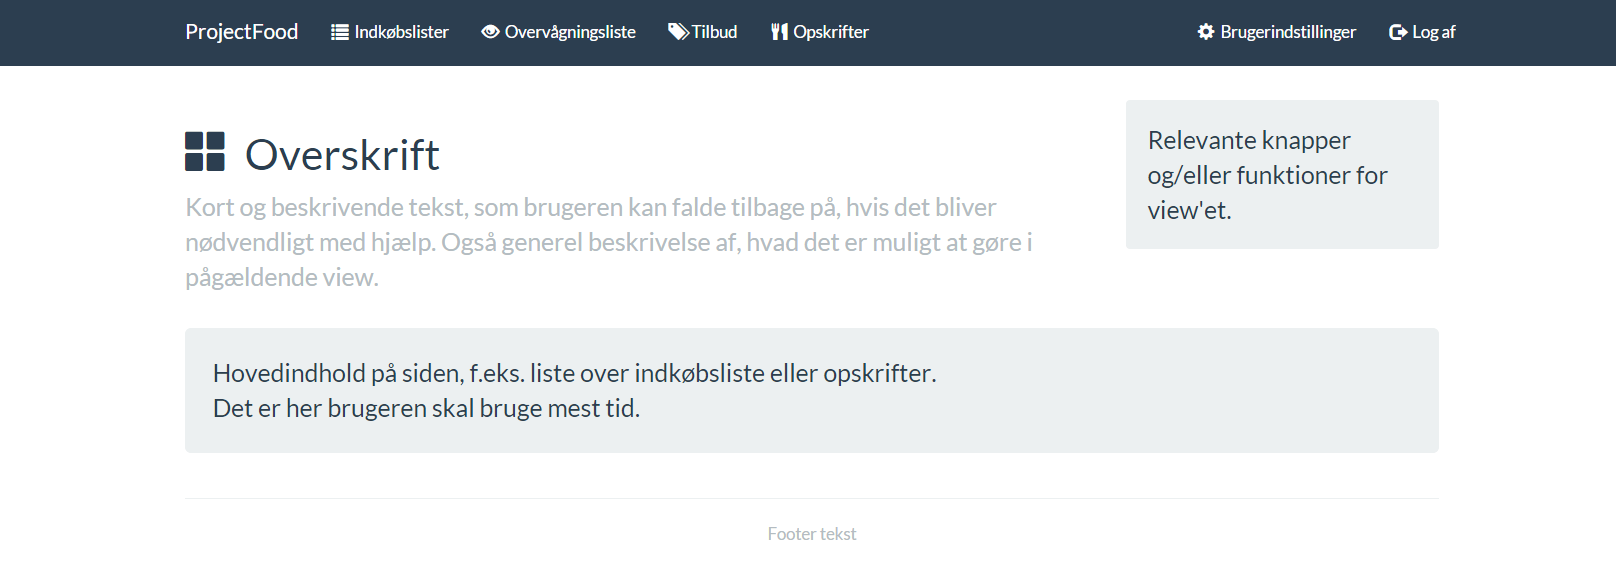
\includegraphics[trim=3.5cm 0cm 3cm 0cm, clip=true, width=1\textwidth]{images/Images/generelt_layout.png}
\caption{Design skabelon som beskriver den umiddelbare inddeling af views i systemet.}\label{ss:design_skabelon}
\end{figure}
Skabelonen er simpelt bygget op med tre hoved grupper, foruden navigerings-baren og footeren. En gruppe til ikon(glyphicon), overskrift og forklarende hjælpetekst, en anden gruppe til knapper og relevante funktioner (det kunne f.eks. være en ``Opret indkøbsliste''-knap), og en tredje gruppe til selve hovedindholdet.
I HTML syntaks vil \myref{ss:design_skabelon}, se således ud:
\begin{lstlisting}[language=HTML, caption=HTML-kode med de tre hoved grupper, label=html:design_skabelon]
<div class="page-header nopadding-xs">
    <div class="container-fluid nopadding">
        <div class="col-md-9 col-xs-12 nopadding">
            <!--- Første gruppe --->
            <h1><span class="glyphicon glyphicon-th-large"></span>&nbsp;&nbsp;Overskrift</h1>
            <p class="hidden-xs lead text-muted nopadding">
                Kort og beskrivende tekst, som brugeren kan falde tilbage på, hvis det bliver nødvendligt med hjælp.
                Også generel beskrivelse af, hvad det er muligt at gøre i pågældende view.
            </p>
            <!--- Første gruppe slut --->
        </div>
        <div class="col-md-3 col-xs-12 nopadding">
            <!--- Anden gruppe --->            
            <div class="well lead">
                Relevante knapper og/eller funktioner for view'et.
            </div>
            <!--- Anden gruppe slut --->
        </div>
    </div>
</div>
<div class="container-fluid nopadding">
    <!--- Tredje gruppe --->
    <div class="well well-lg lead">
        Hovedindhold på siden, f.eks. liste over indkøbsliste eller opskrifter.<br />
        Det er her brugeren skal bruge mest tid.
    </div>
    <!--- Tredje gruppe slut --->
</div>
\end{lstlisting}

I HTML koden i \myref{html:design_skabelon} ses også nogle forskellige bootstrap klasser, der gør, at resultatet bliver det, der kan ses \myref{ss:design_skabelon}. 
Vi udnytter gitter-systemet, som bootstrap stiller til rådighed, og for at få indholdet til at stå, som vi vil have det, og samtidigt se pænt ud på mobil-platform, har vi bl.a. vores egne CSS-klasser som f.eks. \texttt{nopadding}. 
Med denne blanding af bootstrap og vores eget CSS, kan vi tilpasse systemet præcis som vi vil. 
En af de andre funktioner, vi benytter fra bootstrap, er ``glyphicons'', der giver vores system en skub imod mere consistency og affordance, i og med ikonet beskriver overskriften, samt er ens fra navigerings-baren.

\textbf{Mobil tilpasning}\hfill\\
Det meste af vores tilpasning til mobil-platformen, klares af bootstaps responsive design, som de opnår ved at definere forskellige atributter for forskellige skærm størrelser.
Derudover benytter vi os af CSS-klasser, fra bootstrap, som kan skjule og/eller vise ting ved netop forskellige skærm størrelser.

\subsection{Konklusion}